\section{若干函数空间}
\label{sec:ch1-function-spaces}

\subsection*{引言}

本章研究定常 Stokes 方程, 即 Navier--Stokes 方程的定常线性化形式. Stokes 方程的研究本身具有意义, 同时也使我们有机会引入处理完整 Navier--Stokes 方程所需的若干工具.

在第 \ref{sec:ch1-function-spaces} 节中, 我们考虑若干函数空间, 即分量属于 $L^2$ 的无散向量函数空间. 第 \ref{sec:ch1-stokes-existence-uniqueness} 节给出 Stokes 方程的变分表述, 并利用投影定理证明解的存在性与唯一性. 在第 \ref{sec:ch1-stokes-discretization-i} 节和第 \ref{sec:ch1-stokes-discretization-ii} 节中, 我们回顾赋范空间和变分线性方程逼近的若干定义与结果. 随后提出无散向量函数的一个基本空间 $V$ 的几类逼近, 其中包括有限差分逼近以及协调和非协调有限元逼近. 第 \ref{sec:ch1-numerical-algorithms} 节讨论 Stokes 方程的若干逼近算法及相应的离散方程. 这些算法旨在克服条件 $\operatorname{div}u=0$ 所造成的困难. 正如后文将表明的, 有时这一困难并不能仅靠离散化解决.

最后, 第 \ref{sec:ch1-penalty-method} 节研究微可压缩流体的线性化方程, 以及它们向不可压缩流体线性方程(即 Stokes 方程)的渐近收敛.

本节引入并研究若干基本函数空间. 这些结果对后文十分重要, 但本节使用的方法不会再次出现, 因此读者可以略读证明, 只需保留第 \ref{subsec:ch1-notation} 小节所述的一般记号和注 \ref{rem:ch1-summary-results} 中汇总的结果.

\subsection{记号}
\label{subsec:ch1-notation}

在 Euclidean 空间 $\mathbb{R}^n$ 中, 记
\[
e_1=(1,0,\ldots,0),\quad e_2=(0,1,0,\ldots,0),\quad\ldots,\quad e_n=(0,\ldots,0,1)
\]
为标准基, 并以 $x=(x_1,\ldots,x_n)$, $y=(y_1,\ldots,y_n)$, $z=(z_1,\ldots,z_n),\ldots$ 表示该空间中的点.

微分算子
\[
\frac{\partial}{\partial x_i}\qquad(1\leq i\leq n)
\]
记为 $D_i$. 若 $j=(j_1,\ldots,j_n)$ 是多重指标, 则 $D^j$ 表示微分算子
\begin{equation}
D^j=D_1^{j_1}\cdots D_n^{j_n}
=\frac{\partial^{[j]}}{\partial x_1^{j_1}\cdots\partial x_n^{j_n}},
\label{eq:ch1-multi-index-derivative}
\end{equation}
其中
\begin{equation}
[j]=j_1+\cdots+j_n.
\label{eq:ch1-multi-index-order}
\end{equation}
若对某个 $i$ 有 $j_i=0$, 则 $D_i^{j_i}$ 是恒等算子; 特别地, 若 $[j]=0$, 则 $D^j$ 是恒等算子.

\paragraph{集合 $\Omega$.}
设 $\Omega$ 是 $\mathbb{R}^n$ 中边界为 $\Gamma$ 的开集. 一般而言, 我们需要 $\Omega$ 具有某种光滑性. 有时假设 $\Omega$ 在下述意义下光滑:
\begin{equation}
\begin{minipage}{0.72\textwidth}
边界 $\Gamma$ 是 $C^r$ 类的 $(n-1)$ 维流形, 其中 $r\geq1$ 且须具体指定, 并且 $\Omega$ 局部位于 $\Gamma$ 的一侧.
\end{minipage}
\label{eq:ch1-domain-cr-condition}
\end{equation}
称满足 \eqref{eq:ch1-domain-cr-condition} 的集合 $\Omega$ 为 $C^r$ 类集合. 然而, 对实际情形(例如正方形区域中的流动), 这一假设过强, 因此所有主要结果都将在较弱的条件下证明:
\begin{equation}
\begin{minipage}{0.72\textwidth}
$\Omega$ 的边界局部为 Lipschitz 的, 并且 $\Omega$ 局部位于 $\Gamma$ 的一侧.
\end{minipage}
\label{eq:ch1-domain-lipschitz-condition}
\end{equation}
这意味着在任意点 $x\in\Gamma$ 的一个邻域内, $\Gamma$ 可表示为超曲面 $y_n=\theta(y_1,\ldots,y_{n-1})$, 其中 $\theta$ 是 Lipschitz 函数, 而 $(y_1,\ldots,y_n)$ 是 $\mathbb{R}^n$ 中某一基下的直角坐标, 该基可以不同于标准基 $e_1,\ldots,e_n$.

显然, 若 $\Omega$ 为 $C^1$ 类, 则 $\Omega$ 局部为 Lipschitz 的. 对本节后文, 需要注意满足 \eqref{eq:ch1-domain-lipschitz-condition} 的集合 $\Omega$ 是``局部星形的''. 这意味着对每个 $x_j\in\Gamma$, 都存在一个开邻域 $O_j$, 使 $O'_j=\Omega\cap O_j$ 关于其中某一点为星形. 根据 \eqref{eq:ch1-domain-lipschitz-condition}, 还可假设 $O'_j$ 的边界为 Lipschitz 的. 若 $\Gamma$ 有界, 则可由有限族这样的集合 $O_j$, $j\in J$, 覆盖; 若 $\Gamma$ 无界, 则族 $(O_j)_{j\in J}$ 可取为局部有限族.

除非明确说明 $\Omega$ 是 $\mathbb{R}^n$ 中任意开集, 或要求其他光滑性, 否则始终假设 $\Omega$ 满足 \eqref{eq:ch1-domain-lipschitz-condition}.

\begin{figure}[htbp]
\centering
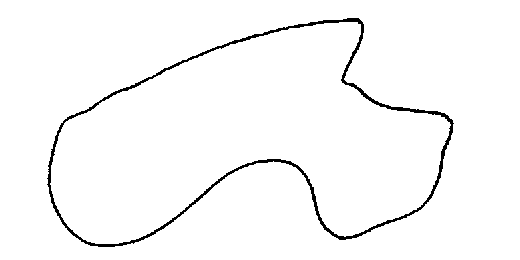
\includegraphics[width=0.42\textwidth]{figures/chapter01-figure01.png}
\caption{}
\label{fig:ch1-domain-example}
\end{figure}

\paragraph{$L^p$ 空间与 Sobolev 空间.}
设 $\Omega$ 是 $\mathbb{R}^n$ 中任意开集. 以 $L^p(\Omega)$, $1<p<+\infty$(或 $L^\infty(\Omega)$), 表示在 $\Omega$ 上定义的实函数空间, 其 $p$ 次幂关于 Lebesgue 测度 $dx=dx_1\cdots dx_n$ 绝对可积(或函数本质有界). 这是 Banach 空间, 范数为
\begin{equation}
\lVert u\rVert_{L^p(\Omega)}
=\left(\int_\Omega\lvert u(x)\rvert^p\,dx\right)^{1/p}.
\label{eq:ch1-lp-norm}
\end{equation}
当 $p=\infty$ 时,
\[
\lVert u\rVert_{L^\infty(\Omega)}=\operatorname*{ess\,sup}_\Omega\lvert u(x)\rvert.
\]
当 $p=2$ 时, $L^2(\Omega)$ 是 Hilbert 空间, 其内积为
\begin{equation}
(u,v)=\int_\Omega u(x)v(x)\,dx.
\label{eq:ch1-l2-inner-product}
\end{equation}

Sobolev 空间 $W^{m,p}(\Omega)$ 是由 $L^p(\Omega)$ 中所有不超过 $m$ 阶的分布导数仍属于 $L^p(\Omega)$ 的函数组成的空间, 其中 $m$ 是整数且 $1\leq p\leq+\infty$. 这是 Banach 空间, 范数为
\begin{equation}
\lVert u\rVert_{W^{m,p}(\Omega)}
=\left(\sum_{[j]\leq m}\lVert D^ju\rVert_{L^p(\Omega)}^p\right)^{1/p}.
\label{eq:ch1-sobolev-norm}
\end{equation}
当 $p=2$ 时, $W^{m,2}(\Omega)=H^m(\Omega)$ 是 Hilbert 空间, 其内积为
\begin{equation}
((u,v))_{H^m(\Omega)}=\sum_{[j]\leq m}(D^ju,D^jv).
\label{eq:ch1-sobolev-inner-product}
\end{equation}

以 $\mathcal{D}(\Omega)$(或 $\mathcal{D}(\overline\Omega)$)表示支集紧含于 $\Omega$(或 $\overline\Omega$)的 $C^\infty$ 函数空间. $\mathcal{D}(\Omega)$ 在 $W^{m,p}(\Omega)$ 中的闭包记为 $W_0^{m,p}(\Omega)$; 当 $p=2$ 时记为 $H_0^m(\Omega)$. 必要时将回顾这些空间的经典性质, 例如稠密性和迹定理, 此时须对 $\Omega$ 作适当正则性假设.

我们经常处理分量属于上述某个空间的 $n$ 维向量函数. 采用记号
\[
\mathbf{L}^p(\Omega)=\{L^p(\Omega)\}^n,\quad
\mathbf{W}^{m,p}(\Omega)=\{W^{m,p}(\Omega)\}^n,
\]
\[
\mathbf{H}^m(\Omega)=\{H^m(\Omega)\}^n,\quad
\mathbf{\mathcal D}(\Omega)=\{\mathcal D(\Omega)\}^n,
\]
并假设这些积空间配备通常的积范数或一个等价范数, 但 $\mathcal D(\Omega)$ 和 $\mathcal D(\overline\Omega)$ 不是赋范空间. 下列空间将频繁出现:
\[
L^2(\Omega),\quad\mathbf L^2(\Omega),\quad H_0^1(\Omega),\quad\mathbf H_0^1(\Omega).
\]
在 $L^2(\Omega)$ 或 $\mathbf L^2(\Omega)$ 上, 内积和范数分别记为 $(\cdot,\cdot)$ 和 $\lvert\cdot\rvert$; 在 $H_0^1(\Omega)$ 或 $\mathbf H_0^1(\Omega)$ 上, 也可分别记为 $[\cdot,\cdot]$ 和 $[\cdot]$.

回顾如下事实: 若 $\Omega$ 在某一方向上有界\footnote{即 $\Omega$ 位于一个板层内, 其边界是与该方向正交的两个超平面. 这对超平面的最小距离称为 $\Omega$ 在相应方向上的厚度.}, 则 Poincaré 不等式成立:
\begin{equation}
\lVert u\rVert_{L^2(\Omega)}\leq c(\Omega)\lVert Du\rVert_{L^2(\Omega)},
\qquad\forall u\in H_0^1(\Omega),
\label{eq:ch1-poincare-inequality}
\end{equation}
其中 $D$ 是该方向上的导数, $c(\Omega)$ 是只依赖于 $\Omega$ 的常数, 并且不超过 $2l$; 这里 $l$ 是 $\Omega$ 的直径, 或 $\Omega$ 在任一方向上的厚度. 此时 $H_0^1(\Omega)$(或 $\mathbf H_0^1(\Omega)$)上的范数 $[\cdot]$ 等价于范数
\begin{equation}
\lVert u\rVert=\left(\sum_{i=1}^n\lvert D_i u\rvert^2\right)^{1/2}.
\label{eq:ch1-h01-gradient-norm}
\end{equation}
$H_0^1(\Omega)$(或 $\mathbf H_0^1(\Omega)$)也是 Hilbert 空间, 相应内积为
\begin{equation}
((u,v))=\sum_{i=1}^n(D_i u,D_i v).
\label{eq:ch1-h01-gradient-inner-product}
\end{equation}
在 $H_0^1(\Omega)$ 和 $\mathbf H_0^1(\Omega)$ 上, 该内积与范数记为 $((\cdot,\cdot))$ 和 $\lVert\cdot\rVert$, 其中 $\Omega$ 在某一方向上有界.

设 $\mathcal V$ 是不附加拓扑的空间
\begin{equation}
\mathcal V=\{u\in\mathbf{\mathcal D}(\Omega):\operatorname{div}u=0\}.
\label{eq:ch1-test-divergence-free-space}
\end{equation}
$\mathcal V$ 在 $\mathbf L^2(\Omega)$ 和 $\mathbf H_0^1(\Omega)$ 中的闭包是 Navier--Stokes 方程研究中的两个基本空间, 分别记为 $H$ 和 $V$. 本节结果将给出 $H$ 与 $V$ 的刻画.

\subsection{一个稠密性定理}
\label{subsec:ch1-density-theorem}

设辅助空间
\[
E(\Omega)=\{u\in\mathbf L^2(\Omega):\operatorname{div}u\in L^2(\Omega)\}.
\]
赋予它内积
\begin{equation}
((u,v))_{E(\Omega)}=(u,v)+(\operatorname{div}u,\operatorname{div}v).
\label{eq:ch1-e-space-inner-product}
\end{equation}
显然, \eqref{eq:ch1-e-space-inner-product} 是 $E(\Omega)$ 上的内积, 且容易看出 $E(\Omega)$ 关于相应范数
\[
\lVert u\rVert_{E(\Omega)}=\{((u,u))_{E(\Omega)}\}^{1/2}
\]
完备\footnote{若 $(u_m)$ 是 $E(\Omega)$ 中的 Cauchy 序列, 则它也是 $\mathbf L^2(\Omega)$ 中的 Cauchy 序列; $u_m$ 收敛到某个 $u\in\mathbf L^2(\Omega)$, 而 $\operatorname{div}u_m$ 收敛到某个 $g\in L^2(\Omega)$. 必有 $g=\operatorname{div}u$, 因而 $u\in E(\Omega)$ 且 $u_m$ 在 $E(\Omega)$ 中收敛到 $u$.}.

我们的目标是证明一个迹定理: 对 $u\in E(\Omega)$, 可以定义其法向分量 $u\cdot\nu$ 在 $\Gamma$ 上的值, 其中 $\nu$ 是边界单位法向量. 所用方法是经典的 Lions--Magenes 方法. 首先证明下述定理.

\MBSourceStatementNumber{theorem}{1}
\begin{Theorem}
\label{thm:ch1-density-in-e}
设 $\Omega$ 是 $\mathbb R^n$ 中的 Lipschitz 开集. 则属于 $\mathbf{\mathcal D}(\overline\Omega)$ 的向量函数在 $E(\Omega)$ 中稠密.
\end{Theorem}

\begin{Proof}
任取 $u\in E(\Omega)$. 我们须证明 $u$ 是 $\mathbf{\mathcal D}(\overline\Omega)$ 中向量函数在 $E(\Omega)$ 中的极限.

(i) 当 $\Omega$ 无界时, 先用 $E(\Omega)$ 中在 $\overline\Omega$ 内具有紧支集(即有界支集)的函数逼近 $u$.

取 $\phi\in\mathcal D(\mathbb R^n)$, 满足 $0\leq\phi\leq1$, 当 $\lvert x\rvert\leq1$ 时 $\phi=1$, 当 $\lvert x\rvert\geq2$ 时 $\phi=0$. 对 $a>0$, 令 $\phi_a$ 为函数 $x\mapsto\phi(x/a)$ 在 $\Omega$ 上的限制. 容易验证 $\phi_a u\in E(\Omega)$, 且当 $a\to\infty$ 时 $\phi_a u$ 在该空间中收敛到 $u$. 因而有界支集函数构成 $E(\Omega)$ 的稠密子空间, 可假设 $u$ 有有界支集.

(ii) 先考虑 $\Omega=\mathbb R^n$ 的情形; 此时 $u\in E(\mathbb R^n)$ 且 $u$ 有紧支集.

利用正则化证明该结果. 取 $\rho\in\mathcal D(\mathbb R^n)$ 为具有紧支集的光滑 $C^\infty$ 函数, 满足 $\rho\geq0$ 且 $\int_{\mathbb R^n}\rho(x)\,dx=1$. 对 $\varepsilon\in(0,1)$, 令 $\rho_\varepsilon(x)=\varepsilon^{-n}\rho(x/\varepsilon)$. 当 $\varepsilon\to0$ 时, $\rho_\varepsilon$ 在分布意义下收敛到 Dirac 分布, 并有经典结果
\begin{equation}
\rho_\varepsilon*v\longrightarrow v\quad\text{在 }L^2(\mathbb R^n)\text{ 中},
\qquad\forall v\in L^2(\mathbb R^n).
\label{eq:ch1-mollifier-l2-convergence}
\end{equation}
这里 $*$ 是卷积算子:
\[
(f*g)(x)=\int_{\mathbb R^n}f(x-y)g(y)\,dy.
\]
若 $f\in L^1(\mathbb R^n)$, $g\in L^p(\mathbb R^n)$, $1\leq p<\infty$, 则 $f*g$ 有意义且属于 $L^p(\mathbb R^n)$.

由于 $\rho_\varepsilon*u$ 有紧支集且各分量为 $C^\infty$ 函数, 它属于 $\mathbf{\mathcal D}(\mathbb R^n)$. 由 \eqref{eq:ch1-mollifier-l2-convergence}, 当 $\varepsilon\to0$ 时, $\rho_\varepsilon*u$ 在 $\mathbf L^2(\mathbb R^n)$ 中收敛到 $u$, 并且
\[
\operatorname{div}(\rho_\varepsilon*u)
=\rho_\varepsilon*\operatorname{div}u
\longrightarrow\operatorname{div}u
\quad\text{在 }L^2(\mathbb R^n)\text{ 中}.
\]
故 $u$ 是 $\mathbf{\mathcal D}(\mathbb R^n)$ 中函数在 $E(\mathbb R^n)$ 中的极限.

(iii) 对一般情形 $\Omega\neq\mathbb R^n$, 使用 \eqref{eq:ch1-domain-lipschitz-condition} 后的说明: $\Omega$ 局部为星形. 集合 $\Omega$ 与 $(O_j)_{j\in J}$ 构成 $\overline\Omega$ 的开覆盖. 取从属于该覆盖的单位分解
\begin{equation}
1=\phi+\sum_{j\in J}\phi_j,
\qquad \phi\in\mathcal D(\Omega),\quad\phi_j\in\mathcal D(O_j).
\label{eq:ch1-partition-of-unity}
\end{equation}
于是
\[
u=\phi u+\sum_{j\in J}\phi_j u.
\]
由于 $u$ 的支集在 $\overline\Omega$ 中紧, 上式中的和实际上是有限和.

函数 $\phi u$ 的支集紧含于 $\Omega$, 因而可按 (ii) 证明 $\phi u$ 是 $\mathbf{\mathcal D}(\Omega)$ 中函数在 $E(\Omega)$ 中的极限. 事实上, 将 $\phi u$ 在 $\Omega$ 外延拓为零, 所得函数属于 $E(\mathbb R^n)$; 对充分小的 $\varepsilon$, $\rho_\varepsilon*(\phi u)$ 的支集紧含于 $\Omega$.

现考虑一个不恒为零的函数 $u_j=\phi_j u$. 集合 $O'_j=O_j\cap\Omega$ 关于其中一点为星形; 经 $\mathbb R^n$ 中的平移后, 可假设该点为 $0$. 令 $\sigma_\lambda$, $\lambda\neq0$, 为线性位似变换 $x\mapsto\lambda x$. 由于 $O'_j$ 为 Lipschitz 集且关于 $0$ 为星形, 显然
\[
\overline{O'_j}\subset O'_j\subset\sigma_\lambda O'_j\quad(\lambda>1),
\qquad
\overline{\sigma_\lambda O'_j}\subset\sigma_\lambda O'_j\subset O'_j\quad(0<\lambda<1).
\]
以 $\sigma_\lambda\circ v$ 表示函数 $x\mapsto v(\sigma_\lambda(x))$. 由下述引理 \ref{lem:ch1-dilation-distribution}, 当 $\lambda>1$ 且 $\lambda\to1$ 时, $\sigma_\lambda\circ u_j$ 在 $O'_j$ 上的限制在 $E(O'_j)$(或 $E(\Omega)$)中收敛到 $u_j$. 若 $\psi_j\in\mathcal D(\sigma_\lambda(O'_j))$ 且在 $O'_j$ 上 $\psi_j=1$, 则函数 $\psi_j(\sigma_\lambda\circ u)$ 显然属于 $E(\mathbb R^n)$. 因而, 只需将 $u_j$ 替换为 $E(\Omega)$ 中某个函数 $v^j$, 它是 $E(\mathbb R^n)$ 中一个具有紧支集的函数 $w^j$ 在 $\Omega$ 上的限制; 可取 $w^j=\psi_j(\sigma_\lambda\circ u)$. 结论于是由 (ii) 得到.
\end{Proof}

还需证明下述引理, 它既给出上述证明中使用的若干结果, 也给出后文所需的其他结果.

\MBSourceStatementNumber{lemma}{1}
\begin{Lemma}
\label{lem:ch1-dilation-distribution}
设 $O$ 是关于 $0$ 为星形的开集.

(i) 若 $p\in\mathcal D'(O)$ 是 $O$ 上的分布, 则可由
\begin{equation}
\langle\sigma_\lambda\circ p,\phi\rangle
=\frac{1}{\lambda^n}\langle p,\sigma_{1/\lambda}\circ\phi\rangle,
\qquad\forall\phi\in\mathcal D(\sigma_\lambda O),\quad\lambda>0,
\label{eq:ch1-dilated-distribution-definition}
\end{equation}
在 $\mathcal D'(\sigma_\lambda O)$ 中定义分布 $\sigma_\lambda\circ p$. $\sigma_\lambda\circ p$ 的导数与 $p$ 的导数满足
\begin{equation}
D_i(\sigma_\lambda\circ p)=\lambda\sigma_\lambda\circ(D_i p),
\qquad1\leq i\leq n.
\label{eq:ch1-dilated-distribution-derivative}
\end{equation}
当 $\lambda>1$ 且 $\lambda\to1$ 时, $\sigma_\lambda\circ p$ 在 $O$ 上的限制在分布意义下收敛到 $p$.

(ii) 若 $p\in L^\alpha(O)$, $1\leq\alpha<+\infty$, 则 $\sigma_\lambda\circ p\in L^\alpha(\sigma_\lambda O)$. 当 $\lambda>1$ 且 $\lambda\to1$ 时, $\sigma_\lambda\circ p$ 在 $O$ 上的限制在 $L^\alpha(O)$ 中收敛到 $p$.
\end{Lemma}

\begin{Proof}
(i) 显然, 映射 $\phi\mapsto\lambda^{-n}\langle p,\sigma_{1/\lambda}\circ\phi\rangle$ 在 $\mathcal D(\sigma_\lambda O)$ 上线性连续, 因而定义了记为 $\sigma_\lambda\circ p$ 的分布. 公式 \eqref{eq:ch1-dilated-distribution-derivative} 由
\begin{align*}
\langle D_i(\sigma_\lambda\circ p),\phi\rangle
&=-\langle\sigma_\lambda\circ p,D_i\phi\rangle
=-\frac1{\lambda^n}\langle p,\sigma_{1/\lambda}\circ(D_i\phi)\rangle\\
&=-\frac1{\lambda^{n-1}}\langle p,D_i(\sigma_{1/\lambda}\circ\phi)\rangle
=\frac1{\lambda^{n-1}}\langle D_i p,\sigma_{1/\lambda}\circ\phi\rangle\\
&=\lambda\langle\sigma_\lambda\circ D_i p,\phi\rangle
\end{align*}
立即得到. 当 $\lambda>1$ 且 $\lambda\to1$ 时, 对充分小的 $\lambda-1$, 函数 $\sigma_{1/\lambda}\circ\phi$ 的支集紧含于 $O$, 且当 $\lambda\to1$ 时在 $\mathcal D(O)$ 中收敛到 $\phi$.

(ii) 显然
\[
\int_{\sigma_\lambda O}\lvert(\sigma_\lambda p)(y)\rvert^\alpha\,dy
=\lambda^n\int_O\lvert p(x)\rvert^\alpha\,dx,
\qquad
\lVert\sigma_\lambda\circ p\rVert_{L^\alpha(\sigma_\lambda O)}
=\lambda^{n/\alpha}\lVert p\rVert_{L^\alpha(O)}.
\]
因此只需对 $L^\alpha(O)$ 的某个稠密子空间中的 $p$ 证明其在 $O$ 上的限制收敛到 $p$. 由于 $\mathcal D(O)$ 在 $L^\alpha(O)$ 中稠密, 而 $p\in\mathcal D(O)$ 时结论显然成立, 证明完成.
\end{Proof}

\subsection{一个迹定理}
\label{subsec:ch1-trace-theorem}

本小节假设 $\Omega$ 是 $C^2$ 类有界开集. 已知存在连续线性算子 $\gamma_0\in\mathcal L(H^1(\Omega),L^2(\Gamma))$(迹算子), 使每个在 $\overline\Omega$ 上二次连续可微的 $u\in H^1(\Omega)$ 满足 $\gamma_0u=u|_\Gamma$. 空间 $H_0^1(\Omega)$ 等于 $\gamma_0$ 的核. 像空间 $\gamma_0(H^1(\Omega))$ 是 $L^2(\Gamma)$ 的稠密子空间, 记为 $H^{1/2}(\Gamma)$; 可赋予它由 $\gamma_0$ 从 $H^1(\Omega)$ 携带而来的范数. 此外存在连续线性算子 $\ell_\Omega\in\mathcal L(H^{1/2}(\Gamma),H^1(\Omega))$(提升算子), 使 $\gamma_0\circ\ell_\Omega$ 是 $H^{1/2}(\Gamma)$ 上的恒等算子. 这些结果见 Lions [1] 和 Lions--Magenes [1].

我们要对 $E(\Omega)$ 中的向量函数证明类似结果. 令 $H^{-1/2}(\Gamma)$ 为 $H^{1/2}(\Gamma)$ 的对偶空间. 由于 $H^{1/2}(\Gamma)\subset L^2(\Gamma)$ 且拓扑更强, 故 $L^2(\Gamma)$ 包含于 $H^{-1/2}(\Gamma)$ 且拓扑更强. 有如下迹定理, 即当 $u\in E(\Omega)$ 时可以定义 $u\cdot\nu|_\Gamma$.

\MBSourceStatementNumber{theorem}{2}
\begin{Theorem}
\label{thm:ch1-normal-trace}
设 $\Omega$ 是 $C^2$ 类有界开集. 则存在连续线性算子 $\gamma_\nu\in\mathcal L(E(\Omega),H^{-1/2}(\Gamma))$, 使
\begin{equation}
\gamma_\nu u=(u\cdot\nu)|_\Gamma,
\qquad\forall u\in\mathbf{\mathcal D}(\overline\Omega).
\label{eq:ch1-normal-trace-smooth}
\end{equation}
对所有 $u\in E(\Omega)$ 和 $w\in H^1(\Omega)$, 下述广义 Stokes 公式成立:
\begin{equation}
(u,\operatorname{grad}w)+(\operatorname{div}u,w)
=\langle\gamma_\nu u,\gamma_0w\rangle.
\label{eq:ch1-generalized-stokes-formula}
\end{equation}
\end{Theorem}

\begin{Proof}
取 $\phi\in H^{1/2}(\Gamma)$, 并取满足 $\gamma_0w=\phi$ 的 $w\in H^1(\Omega)$. 对 $u\in E(\Omega)$, 定义
\[
X_u(\phi)=\int_\Omega\{\operatorname{div}u(x)w(x)+u(x)\cdot\operatorname{grad}w(x)\}\,dx
=(\operatorname{div}u,w)+(u,\operatorname{grad}w).
\]

\MBSourceStatementNumber{lemma}{2}
\begin{Lemma}
\label{lem:ch1-trace-functional-independent}
只要 $w\in H^1(\Omega)$ 且 $\gamma_0w=\phi$, $X_u(\phi)$ 就与 $w$ 的选择无关.
\end{Lemma}

\begin{Proof}
设 $w_1,w_2\in H^1(\Omega)$ 且 $\gamma_0w_1=\gamma_0w_2=\phi$, 并令 $w=w_1-w_2$. 我们须证明
\begin{equation}
(\operatorname{div}u,w)+(u,\operatorname{grad}w)=0.
\label{eq:ch1-trace-functional-zero}
\end{equation}
由于 $w\in H^1(\Omega)$ 且 $\gamma_0w=0$, 故 $w\in H_0^1(\Omega)$, 并且它是紧支集光滑函数在 $H^1(\Omega)$ 中的极限: $w=\lim_m w_m$, $w_m\in\mathcal D(\Omega)$. 对每个 $w_m\in\mathcal D(\Omega)$, 显然有
\[
(\operatorname{div}u,w_m)+(u,\operatorname{grad}w_m)=0.
\]
令 $m\to\infty$ 即得 \eqref{eq:ch1-trace-functional-zero}.
\end{Proof}

现取 $w=\ell_\Omega\phi$. 由 Schwarz 不等式,
\[
\lvert X_u(\phi)\rvert\leq\lVert u\rVert_{E(\Omega)}\lVert w\rVert_{H^1(\Omega)}.
\]
又因 $\ell_\Omega\in\mathcal L(H^{1/2}(\Gamma),H^1(\Omega))$,
\begin{equation}
\lvert X_u(\phi)\rvert
\leq c_0\lVert u\rVert_{E(\Omega)}\lVert\phi\rVert_{H^{1/2}(\Gamma)},
\label{eq:ch1-trace-functional-bound}
\end{equation}
其中 $c_0$ 是线性算子 $\ell_\Omega$ 的范数. 因而映射 $\phi\mapsto X_u(\phi)$ 是从 $H^{1/2}(\Gamma)$ 到 $\mathbb R$ 的连续线性映射. 所以存在 $g=g(u)\in H^{-1/2}(\Gamma)$, 使
\begin{equation}
X_u(\phi)=\langle g,\phi\rangle.
\label{eq:ch1-normal-trace-duality-definition}
\end{equation}
映射 $u\mapsto g(u)$ 显然线性, 且由 \eqref{eq:ch1-trace-functional-bound},
\begin{equation}
\lVert g\rVert_{H^{-1/2}(\Gamma)}
\leq c_0\lVert u\rVert_{E(\Omega)}.
\label{eq:ch1-normal-trace-bound}
\end{equation}
这证明映射 $u\mapsto g(u)=\gamma_\nu u$ 从 $E(\Omega)$ 到 $H^{-1/2}(\Gamma)$ 连续. 由 $\gamma_\nu u$ 的定义, \eqref{eq:ch1-generalized-stokes-formula} 直接成立, 最后只须证明 \eqref{eq:ch1-normal-trace-smooth}.

\MBSourceStatementNumber{lemma}{3}
\begin{Lemma}
\label{lem:ch1-normal-trace-smooth}
若 $u\in\mathbf{\mathcal D}(\overline\Omega)$, 则 $\gamma_\nu u$ 等于 $u\cdot\nu$ 在 $\Gamma$ 上的限制.
\end{Lemma}

\par\vspace{0.1cm}\noindent\textbf{证明:}\quad
对这样的光滑函数 $u$ 和任意 $w\in\mathcal D(\overline\Omega)$(或者当 $u,w$ 在 $\overline\Omega$ 上二次连续可微时), 由 Stokes 公式,
\begin{align*}
X_u(\gamma_0w)
&=\int_\Omega\operatorname{div}(uw)\,dx
=\int_\Gamma w(u\cdot\nu)\,d\Gamma\\
&=\int_\Gamma(u\cdot\nu)(\gamma_0w)\,d\Gamma
=\langle u\cdot\nu,\gamma_0w\rangle.
\end{align*}
对这些 $w$, 其迹 $\gamma_0w$ 在 $H^{1/2}(\Gamma)$ 中稠密, 故由连续性, 对每个 $\phi\in H^{1/2}(\Gamma)$ 都有 $X_u(\phi)=\langle u\cdot\nu,\phi\rangle$. 与 \eqref{eq:ch1-normal-trace-duality-definition} 比较, 得 $\gamma_\nu u=u\cdot\nu|_\Gamma$.
\end{Proof}

\MBSourceStatementNumber{remark}{1}
\begin{Remark}
\label{rem:ch1-normal-trace-uniqueness}
定理 \ref{thm:ch1-density-in-e} 并未在定理 \ref{thm:ch1-normal-trace} 的证明中被显式使用, 但稠密性定理与引理 \ref{lem:ch1-normal-trace-smooth} 结合表明, 算子 $\gamma_\nu$ 是唯一的, 因为它在一个稠密子集上的值已经确定.
\end{Remark}

\MBSourceStatementNumber{remark}{2}
\begin{Remark}
\label{rem:ch1-normal-trace-surjective}
事实上, 算子 $\gamma_\nu$ 将 $E(\Omega)$ 映满 $H^{-1/2}(\Gamma)$.

给定 $\phi\in H^{-1/2}(\Gamma)$ 且 $\langle\phi,1\rangle=0$. Neumann 问题
\begin{equation}
\Delta p=0\quad\text{在 }\Omega\text{ 中},
\qquad \frac{\partial p}{\partial\nu}=\phi\quad\text{在 }\Gamma\text{ 上}
\label{eq:ch1-neumann-lifting-problem}
\end{equation}
存在弱解 $p=p(\phi)\in H^1(\Omega)$, 且在相差一个加性常数的意义下唯一, 见 Lions--Magenes [1]. 对其中一个解 $p$, 令 $u=\operatorname{grad}p$. 显然 $u\in E(\Omega)$ 且 $\gamma_\nu u=\phi$. 此外, 显然存在各分量属于 $C^1(\overline\Omega)$ 的向量函数 $u_0$, 使 $\gamma_\nu u_0=1$. 因而对任意 $\psi\in H^{-1/2}(\Gamma)$, 写成
\begin{equation}
\psi=\phi+\frac{\langle\psi,1\rangle}{\operatorname{meas}\Gamma},
\qquad
\phi=\psi-\frac{\langle\psi,1\rangle}{\operatorname{meas}\Gamma},
\label{eq:ch1-normal-trace-mean-splitting}
\end{equation}
并令
\begin{equation}
u=\operatorname{grad}p(\phi)
+\frac{\langle\psi,1\rangle}{\operatorname{meas}\Gamma}u_0,
\label{eq:ch1-normal-trace-lifting}
\end{equation}
便可定义满足 $\gamma_\nu u=\psi$ 的 $u=u(\psi)$. 而且映射 $\psi\mapsto u(\psi)$ 是从 $H^{-1/2}(\Gamma)$ 到 $E(\Omega)$ 的连续线性映射, 即与 $\ell_\Omega$ 类似的提升算子.
\end{Remark}

令 $E_0(\Omega)$ 为 $\mathbf{\mathcal D}(\Omega)$ 在 $E(\Omega)$ 中的闭包. 有如下结果.

\MBSourceStatementNumber{theorem}{3}
\begin{Theorem}
\label{thm:ch1-kernel-normal-trace}
$\gamma_\nu$ 的核等于 $E_0(\Omega)$.
\end{Theorem}

\begin{Proof}
若 $u\in E_0(\Omega)$, 则由该空间的定义, 存在 $u_m\in\mathbf{\mathcal D}(\Omega)$, 使当 $m\to\infty$ 时 $u_m$ 在 $E(\Omega)$ 中收敛到 $u$. 由定理 \ref{thm:ch1-normal-trace}, $\gamma_\nu u_m=0$, 因而
\[
\gamma_\nu u=\lim_{m\to\infty}\gamma_\nu u_m=0.
\]

反之, 设 $u\in E(\Omega)$ 且 $\gamma_\nu u=0$. 我们证明 $u$ 是 $\mathbf{\mathcal D}(\Omega)$ 中向量函数在 $E(\Omega)$ 中的极限.

任取 $\Phi\in\mathcal D(\mathbb R^n)$, 并令 $\phi$ 为 $\Phi$ 在 $\Omega$ 上的限制. 由 $\gamma_\nu u=0$,
\[
\langle\gamma_\nu u,\gamma_0\phi\rangle=0,
\]
即
\[
\int_\Omega[\operatorname{div}u\,\phi+u\cdot\operatorname{grad}\phi],dx=0.
\]
因此对所有 $\Phi\in\mathcal D(\mathbb R^n)$,
\[
\int_{\mathbb R^n}[(\operatorname{div}u)^+\Phi+u^+\cdot\operatorname{grad}\Phi],dx=0,
\]
从而
\begin{equation}
\operatorname{div}u^+=(\operatorname{div}u)^+,
\label{eq:ch1-zero-extension-divergence}
\end{equation}
其中 $v^+$ 表示在 $\Omega$ 中等于 $v$, 在 $\mathbb R^n\setminus\Omega$ 中等于零的函数. 这说明 $u^+\in E(\mathbb R^n)$.

完全按照定理 \ref{thm:ch1-density-in-e} 的证明步骤, 特别是 (i) 和 (ii), 可将一般情形约化到 $u$ 的支集包含于某个 $O_j\cap\overline\Omega$ 中的情形. 对这样的 $u$, 注意 $u^+\in E(\mathbb R^n)$; 当 $0<\lambda<1$ 时, $\sigma_\lambda\circ u^+$ 的支集紧含于 $O'_j$, 其中 $O'_j$ 假设关于 $0$ 为星形. 由引理 \ref{lem:ch1-dilation-distribution}, 当 $\lambda\to1$ 时, $\sigma_\lambda\circ u^+$ 在 $O'_j$(或 $\Omega$)上的限制在 $E(O'_j)$(或 $E(\Omega)$)中收敛到 $u$. 问题于是约化为以 $\mathcal D(\mathbb R^n)$ 中的元素逼近支集紧含于 $\Omega$ 的函数 $u$, 这可按定理 \ref{thm:ch1-density-in-e} 证明的 (ii) 通过正则化直接得到.
\end{Proof}

\MBSourceStatementNumber{remark}{3}
\begin{Remark}
\label{rem:ch1-nonsmooth-trace}
若 $\Omega$ 无界或其边界不光滑, 某些部分结果仍然成立. 例如, 若 $u\in E(\Omega)$, 则可在 $\Gamma$ 的每个 $C^2$ 类有界部分 $\Gamma_0$ 上定义 $\gamma_\nu u$, 且 $\gamma_\nu u\in H^{-1/2}(\Gamma_0)$. 若 $\Omega$ 光滑但无界, 或其边界是有限个 $C^2$ 类有界 $(n-1)$ 维流形的并, 则可用这种方式在整个 $\Gamma$ 上定义 $\gamma_\nu u$. 然而, 广义 Stokes 公式 \eqref{eq:ch1-generalized-stokes-formula} 此时并不成立.

若对 $H^1(\Omega)$ 中函数的迹知道更多, 结果可以更精确. 假设下列结论成立:

- 存在 $\gamma_0\in\mathcal L(H^1(\Omega),L^2(\Gamma))$, 使每个 $u\in\mathcal D(\overline\Omega)$ 满足 $\gamma_0u=u|_\Gamma$. 记 $\gamma_0(H^1(\Omega))$ 为 $\mathcal H^{1/2}(\Gamma)$;

- 存在提升算子 $\ell_\Omega\in\mathcal L(\mathcal H^{1/2}(\Gamma),H^1(\Omega))$, 使 $\gamma_0\circ\ell_\Omega$ 为恒等算子; $\mathcal H^{1/2}(\Gamma)$ 配备由 $\gamma_0$ 携带的范数;

- $\Omega$ 是 Lipschitz 集.

则前述所有结果均可推广到这一情形. 定理 \ref{thm:ch1-density-in-e} 和定理 \ref{thm:ch1-kernel-normal-trace} 成立. 定理 \ref{thm:ch1-normal-trace} 的证明把 $\gamma_\nu u$ 定义为 $\mathcal H^{-1/2}(\Gamma)$ 中的元素, 其中 $\mathcal H^{-1/2}(\Gamma)$ 是 $\mathcal H^{1/2}(\Gamma)$ 的对偶空间. 广义 Stokes 公式 \eqref{eq:ch1-generalized-stokes-formula} 有效.
\end{Remark}

\subsection{空间 \texorpdfstring{$H$ 与 $V$}{H 与 V} 的刻画}
\label{subsec:ch1-characterization-h-v}

回顾第 \ref{subsec:ch1-notation} 小节末尾的记号:
\[
\mathcal V=\{u\in\mathbf{\mathcal D}(\Omega):\operatorname{div}u=0\},
\]
\[
H=\mathcal V\text{ 在 }\mathbf L^2(\Omega)\text{ 中的闭包},
\qquad
V=\mathcal V\text{ 在 }\mathbf H_0^1(\Omega)\text{ 中的闭包}.
\]

\paragraph{分布梯度的刻画.}
设 $\Omega$ 是 $\mathbb R^n$ 中的开集, $p\in\mathcal D'(\Omega)$ 是 $\Omega$ 上的分布. 容易验证, 对任意 $v\in\mathcal V$,
\begin{equation}
\langle\operatorname{grad}p,v\rangle
=\sum_{i=1}^n\langle D_i p,v^i\rangle
=-\sum_{i=1}^n\langle p,D_i v^i\rangle
=-\langle p,\operatorname{div}v\rangle=0.
\label{eq:ch1-gradient-annihilates-v}
\end{equation}
该性质的逆命题也成立. 这一重要性质可利用 de Rham 的一个深刻结果证明\footnote{这里简述超出本书范围的证明. 考虑流 $f=\sum_{i=1}^n f_i\,dx_i$, $f_i\in\mathcal D'(\Omega)$, 以及具有紧支集的 $(n-1)$ 次 $C^\infty$ 形式 $\omega=\sum_{i=1}^n(-1)^iv^i\,dx_1\wedge\cdots\wedge\widehat{dx_i}\wedge\cdots\wedge dx_n$, $v^i\in\mathcal D(\Omega)$. 当且仅当 $v=(v^1,\ldots,v^n)\in\mathcal V$ 时 $d\omega=0$. de Rham [1] 第 114 页的定理 $17'$ 说明, 对 $f\in\mathcal D'(\Omega)$, 当且仅当对上述每个 $\omega$ 都有 $\langle f,\omega\rangle=0$ 时, 存在 $g\in\mathcal D'(\Omega)$ 使 $f=dg$, 即 $f_i=D_i g$. 这等价于命题 \ref{prop:ch1-de-rham-gradient}. 此证明由 J.L. Lions 私下告知. 注 \ref{rem:ch1-alternate-gradient-proof} 给出基于初等论证和命题 \ref{prop:ch1-gradient-regularity} 的另一证明; 另见补充评论. AMS Chelsea 版补注: 现已有不使用流理论或命题 \ref{prop:ch1-gradient-regularity} 的第三种简单自足证明, 见 X. Wang (1993).}.

\MBSourceStatementNumber{proposition}{1}
\begin{Proposition}
\label{prop:ch1-de-rham-gradient}
设 $\Omega$ 是 $\mathbb R^n$ 中的开集, 且 $f=\{f_1,\ldots,f_n\}$, $f_i\in\mathcal D'(\Omega)$, $i=1,\ldots,n$. 存在某个 $p\in\mathcal D'(\Omega)$ 使
\begin{equation}
f=\operatorname{grad}p
\label{eq:ch1-distribution-gradient}
\end{equation}
的充要条件是
\begin{equation}
\langle f,v\rangle=0,
\qquad\forall v\in\mathcal V.
\label{eq:ch1-distribution-gradient-condition}
\end{equation}
\end{Proposition}

该结果对于后文解释 Navier--Stokes 方程及相关方程的变分表述至关重要. 下面陈述若干相关结果.

\MBSourceStatementNumber{proposition}{2}
\begin{Proposition}
\label{prop:ch1-gradient-regularity}
设 $\Omega$ 是 $\mathbb R^n$ 中的有界 Lipschitz 开集.

(i) 若分布 $p$ 的所有一阶导数 $D_i p$, $1\leq i\leq n$, 都属于 $L^2(\Omega)$, 则 $p\in L^2(\Omega)$ 且
\begin{equation}
\lVert p\rVert_{L^2(\Omega)/\mathbb R}
\leq c(\Omega)\lVert\operatorname{grad}p\rVert_{\mathbf L^2(\Omega)}.
\label{eq:ch1-gradient-l2-quotient-bound}
\end{equation}

(ii) 若分布 $p$ 的所有一阶导数 $D_i p$, $1\leq i\leq n$, 都属于 $H^{-1}(\Omega)$, 则 $p\in L^2(\Omega)$ 且
\begin{equation}
\lVert p\rVert_{L^2(\Omega)/\mathbb R}
\leq c(\Omega)\lVert\operatorname{grad}p\rVert_{\mathbf H^{-1}(\Omega)}.
\label{eq:ch1-gradient-hminus1-bound}
\end{equation}
在两种情形中, 若 $\Omega$ 是 $\mathbb R^n$ 中任意开集, 则 $p\in L^2_{\mathrm{loc}}(\Omega)$.
\end{Proposition}

\begin{Proof}
对有界星形开集 $\Omega$, (i) 和 \eqref{eq:ch1-gradient-l2-quotient-bound} 由 Deny--Lions [1] 证明. 在当前情形下, 由该结果, $p$ 在每个闭包包含于 $\Omega$ 的球以及 \eqref{eq:ch1-domain-lipschitz-condition} 后定义的所有集合 $O'_j$ 上属于 $L^2$. 有限个这样的球和集合 $O'_j$ 覆盖 $\Omega$, 故结论成立.

若 $\Omega$ 为 $C^1$ 类, (ii) 由 Magenes--Stampacchia [1] 证明; 当 $\Omega$ 仅为 Lipschitz 集时, 由 J. Nečas [2] 证明.

对不具有任何正则性的集合, 在每个闭包包含于 $\Omega$ 的球上应用上述结果, 只能得到 $p\in L^2_{\mathrm{loc}}(\Omega)$.
\end{Proof}

\MBSourceStatementNumber{remark}{4}
\begin{Remark}
\label{rem:ch1-gradient-operator-range}
(i) 结合命题 \ref{prop:ch1-de-rham-gradient} 与命题 \ref{prop:ch1-gradient-regularity}, 可知若 $f\in\mathbf H^{-1}(\Omega)$(或 $\mathbf L^2_{\mathrm{loc}}(\Omega)$), 且对所有 $v\in\mathcal V$ 有 $(f,v)=0$, 则 $f=\operatorname{grad}p$, 其中 $p\in L^2_{\mathrm{loc}}(\Omega)$. 若 $\Omega$ 还是有界 Lipschitz 开集, 则 $p\in L^2(\Omega)$(或 $H^1(\Omega)$).

(ii) 命题 \ref{prop:ch1-gradient-regularity} 的 (ii) 表明梯度算子是从 $L^2(\Omega)/\mathbb R$ 到 $\mathbf H^{-1}(\Omega)$ 的同构; 因而该线性算子的值域是闭的. 回顾当 $\Omega$ 有界时, $L^2(\Omega)/\mathbb R$ 同构于 $L^2(\Omega)$ 中与常数正交的子空间:
\[
L^2(\Omega)/\mathbb R
=\left\{p\in L^2(\Omega):\int_\Omega p(x)\,dx=0\right\}.
\]
另见 \eqref{eq:ch1-negative-norm-pressure-estimate} 中 \eqref{eq:ch1-gradient-hminus1-bound} 的另一版本.
\end{Remark}

\paragraph{空间 $H$ 的刻画.}
现在可以给出 $H$ 以及它在 $\mathbf L^2(\Omega)$ 中的正交补 $H^\perp$ 的如下刻画.

\MBSourceStatementNumber{theorem}{4}
\begin{Theorem}
\label{thm:ch1-characterization-h}
设 $\Omega$ 是 $\mathbb R^n$ 中有界 Lipschitz 开集. 则
\begin{equation}
H^\perp=\{u\in\mathbf L^2(\Omega):u=\operatorname{grad}p, p\in H^1(\Omega)\},
\label{eq:ch1-h-orthogonal-characterization}
\end{equation}
\begin{equation}
H=\{u\in\mathbf L^2(\Omega):\operatorname{div}u=0, \gamma_\nu u=0\}.
\label{eq:ch1-h-characterization}
\end{equation}
\end{Theorem}

\begin{Proof}
先证明 \eqref{eq:ch1-h-orthogonal-characterization}. 设 $u$ 属于该式右端的空间. 则对所有 $v\in\mathcal V$,
\begin{equation}
(u,v)=(\operatorname{grad}p,v)=-(p,\operatorname{div}v)=0.
\label{eq:ch1-gradient-orthogonal-v}
\end{equation}
故 $u\in H^\perp$.

反之, $H^\perp$ 包含于 \eqref{eq:ch1-h-orthogonal-characterization} 右端的空间. 事实上, 若 $u\in H^\perp$, 则 $(u,v)=0$ 对所有 $v\in\mathcal V$ 成立. 由命题 \ref{prop:ch1-de-rham-gradient}, $u=\operatorname{grad}p$, $p\in\mathcal D'(\Omega)$; 再由命题 \ref{prop:ch1-gradient-regularity}, $p\in H^1(\Omega)$.

再证明 \eqref{eq:ch1-h-characterization}. 令 $H'$ 为该式右端的空间, 先证明 $H\subset H'$. 若 $u\in H$, 则 $u=\lim_{m\to\infty}u_m$, $u_m\in\mathcal V$. 这一 $\mathbf L^2(\Omega)$ 中的收敛蕴含分布意义下的收敛. 由于微分在分布空间中是连续算子且 $\operatorname{div}u_m=0$, 得 $\operatorname{div}u=0$. 因 $\operatorname{div}u_m=\operatorname{div}u=0$, $u_m,u\in E(\Omega)$, 且
\begin{equation}
\lVert u-u_m\rVert_{E(\Omega)}=\lVert u-u_m\rVert_{\mathbf L^2(\Omega)}.
\label{eq:ch1-e-l2-norm-on-divfree}
\end{equation}
所以 $u_m$ 在 $E(\Omega)$ 中收敛到 $u$, 且 $\gamma_\nu u=\lim_{m\to\infty}\gamma_\nu u_m=0$, 因为每个 $u_m\in\mathcal V$ 都有 $u_m\cdot\nu|_\Gamma=0$. 故 $u\in H'$.

若 $H$ 不是整个 $H'$, 令 $H''$ 为 $H$ 在 $H'$ 中的正交补. 由 \eqref{eq:ch1-h-orthogonal-characterization}, 每个 $u\in H''$ 都是某个 $p\in H^1(\Omega)$ 的梯度; 此外 $p$ 满足
\begin{equation}
\Delta p=\operatorname{div}u=0,
\qquad u\cdot\nu|_\Gamma=\left.\frac{\partial p}{\partial\nu}\right|_\Gamma=0.
\label{eq:ch1-harmonic-neumann-zero}
\end{equation}
这蕴含 $p$ 为常数且 $u=0$. 因而 $H''=\{0\}$, 所以 $H=H'$.
\end{Proof}

\MBSourceStatementNumber{remark}{5}
\begin{Remark}
\label{rem:ch1-h-unbounded-domain}
若 $\Omega$ 是 $\mathbb R^n$ 中任意开集, 对 \eqref{eq:ch1-h-orthogonal-characterization} 的证明稍作修改即可得到
\begin{equation}
H^\perp=\{u\in\mathbf L^2(\Omega):u=\operatorname{grad}p, p\in L^2_{\mathrm{loc}}(\Omega)\}.
\label{eq:ch1-h-orthogonal-arbitrary-domain}
\end{equation}
若 $\Omega$ 无界但满足条件 \eqref{eq:ch1-domain-lipschitz-condition}, 则
\begin{equation}
H^\perp=\{u\in\mathbf L^2(\Omega):u=\operatorname{grad}p, p\in L^2_{\mathrm{loc}}(\overline\Omega)\}.
\label{eq:ch1-h-orthogonal-unbounded-lipschitz}
\end{equation}
\end{Remark}

\MBSourceStatementNumber{theorem}{5}
\begin{Theorem}
\label{thm:ch1-helmholtz-decomposition}
设 $\Omega$ 是 $C^2$ 类有界开集. 则
\begin{equation}
\mathbf L^2(\Omega)=H\oplus H_1\oplus H_2,
\label{eq:ch1-l2-orthogonal-decomposition}
\end{equation}
其中 $H,H_1,H_2$ 两两正交, 且
\begin{equation}
H_1=\{u\in\mathbf L^2(\Omega):u=\operatorname{grad}p, p\in H^1(\Omega), \Delta p=0\},
\label{eq:ch1-h1-harmonic-gradient-space}
\end{equation}
\begin{equation}
H_2=\{u\in\mathbf L^2(\Omega):u=\operatorname{grad}p, p\in H_0^1(\Omega)\}.
\label{eq:ch1-h2-dirichlet-gradient-space}
\end{equation}
\end{Theorem}

\begin{Proof}
显然 $H_1,H_2\subset H^\perp$, 且 $H,H_1,H_2$ 中任意两个空间的交均为 $\{0\}$. 空间 $H_1$ 与 $H_2$ 正交. 若 $u=\operatorname{grad}p\in H_1$, $v=\operatorname{grad}q\in H_2$, 则 $u\in E(\Omega)$. 利用广义 Stokes 公式 \eqref{eq:ch1-generalized-stokes-formula},
\[
(u,v)=(u,\operatorname{grad}q)
=\langle\gamma_\nu u,\gamma_0q\rangle-(\operatorname{div}u,q)=0,
\]
因为 $\gamma_0q=0$ 且 $\operatorname{div}u=\Delta p=0$.

还须证明 $\mathbf L^2(\Omega)$ 中任一元素 $u$ 可写为 $H,H_1,H_2$ 中元素 $u_0,u_1,u_2$ 之和. 对这样的 $u$, 令 $p$ 为 Dirichlet 问题
\[
\Delta p=\operatorname{div}u\in H^{-1}(\Omega),
\qquad p\in H_0^1(\Omega)
\]
的唯一解, 并取
\begin{equation}
u_2=\operatorname{grad}p.
\label{eq:ch1-decomposition-u2}
\end{equation}
再令 $q$ 为 Neumann 问题
\begin{equation}
\Delta q=0,
\qquad\left.\frac{\partial q}{\partial\nu}\right|_\Gamma
=\gamma_\nu(u-\operatorname{grad}p)
\label{eq:ch1-decomposition-neumann-q}
\end{equation}
的解. 注意 $\operatorname{div}(u-\operatorname{grad}p)=0$, 故 $u-\operatorname{grad}p\in E(\Omega)$, 而 $\gamma_\nu(u-\operatorname{grad}p)$ 可定义为 $H^{-1/2}(\Gamma)$ 中的元素. 由 Stokes 公式 \eqref{eq:ch1-generalized-stokes-formula},
\[
\langle\gamma_\nu(u-\operatorname{grad}p),1\rangle
=\int_\Omega\operatorname{div}(u-\operatorname{grad}p)\,dx=0.
\]
由 Lions--Magenes [1] 的结果, Neumann 问题 \eqref{eq:ch1-decomposition-neumann-q} 有解, 且在相差一个加性常数的意义下唯一. 取
\begin{equation}
u_1=\operatorname{grad}q,
\label{eq:ch1-decomposition-u1}
\end{equation}
\begin{equation}
u_0=u-u_1-u_2.
\label{eq:ch1-decomposition-u0}
\end{equation}
现证明 $u_0\in H$. 有
\[
\operatorname{div}u_0=\operatorname{div}(u-u_1-u_2)=\operatorname{div}u-\Delta p=0,
\]
以及
\[
\gamma_\nu u_0=\gamma_\nu(u-u_1-u_2)
=\gamma_\nu(u-\operatorname{grad}p)-\frac{\partial q}{\partial\nu}=0.
\]
由定理 \ref{thm:ch1-characterization-h}, $u_0\in H$.
\end{Proof}

\MBSourceStatementNumber{remark}{6}
\begin{Remark}
\label{rem:ch1-summary-results}
(i) 以 $P_H$ 表示 $\mathbf L^2(\Omega)$ 到 $H$ 上的正交投影. 显然 $P_H$ 在 $\mathbf L^2(\Omega)$ 中连续. 事实上, $P_H$ 也将 $\mathbf H^1(\Omega)$ 映入自身, 并关于 $\mathbf H^1(\Omega)$ 的范数连续. 在定理 \ref{thm:ch1-helmholtz-decomposition} 的证明中, 假设 $u\in\mathbf H^1(\Omega)$, 则 $p\in H_0^1(\Omega)\cap H^2(\Omega)$, $u-\operatorname{grad}p\in\mathbf H^1(\Omega)$, 且 $\gamma_\nu(u-\operatorname{grad}p)\in H^{1/2}(\Gamma)$. 最后由 \eqref{eq:ch1-decomposition-neumann-q} 推得 $q\in H^2(\Omega)$, 并有
\[
P_Hu=u-\operatorname{grad}(p+q)\in\mathbf H^1(\Omega).
\]
映射 $u\mapsto p$ 和 $u-\operatorname{grad}p\mapsto q$ 在相应空间中连续, 见 Lions--Magenes [1]. 因而 $P_H$ 从 $\mathbf H^1(\Omega)$ 到自身连续:
\begin{equation}
\lVert P_Hu\rVert_{\mathbf H^1(\Omega)}
\leq c(\Omega)\lVert u\rVert_{\mathbf H^1(\Omega)},
\qquad\forall u\in\mathbf H^1(\Omega).
\label{eq:ch1-helmholtz-projection-h1-bound}
\end{equation}
若 $\Omega$ 为 $C^{r+1}$ 类, 其中整数 $r\geq1$, 类似论证表明, 若 $u\in\mathbf H^r(\Omega)$, 则 $P_Hu\in\mathbf H^r(\Omega)$, 且 $P_H$ 关于 $\mathbf H^r(\Omega)$ 的范数线性连续:
\begin{equation}
\lVert P_Hu\rVert_{\mathbf H^r(\Omega)}
\leq c(r,\Omega)\lVert u\rVert_{\mathbf H^r(\Omega)},
\qquad\forall u\in\mathbf H^r(\Omega).
\label{eq:ch1-helmholtz-projection-hr-bound}
\end{equation}

(ii) 多连通 $\Omega$ 时出现的 $H$ 的一个正交分解见附录 \MBUnresolvedReference{appendix}{I}.
\end{Remark}

\paragraph{空间 $V$ 的刻画.}

\MBSourceStatementNumber{theorem}{6}
\begin{Theorem}
\label{thm:ch1-characterization-v}
设 $\Omega$ 是有界 Lipschitz 开集. 则
\begin{equation}
V=\{u\in\mathbf H_0^1(\Omega):\operatorname{div}u=0\}.
\label{eq:ch1-v-characterization}
\end{equation}
\end{Theorem}

\begin{Proof}
令 $V'$ 为 \eqref{eq:ch1-v-characterization} 右端的空间. 显然 $V\subset V'$. 事实上, 若 $u\in V$, 则 $u=\lim_m u_m$, $u_m\in\mathcal V$; 这一 $\mathbf H_0^1(\Omega)$ 中的收敛蕴含 $\operatorname{div}u_m\to\operatorname{div}u$. 由于 $\operatorname{div}u_m=0$, 得 $\operatorname{div}u=0$.

为证明 $V=V'$, 只须证明 $V'$ 上任何在 $\mathcal V$ 上为零的连续线性泛函 $L$ 恒等于零. 首先注意 $L$ 有如下形式的一个不唯一表示:
\begin{equation}
L(v)=\sum_{i=1}^n\langle\ell_i,v^i\rangle,
\qquad\ell_i\in H^{-1}(\Omega).
\label{eq:ch1-v-functional-representation}
\end{equation}
事实上, $V'$ 是 $\mathbf H_0^1(\Omega)=[H_0^1(\Omega)]^n$ 的闭子空间; $V'$ 上任一连续线性泛函可延拓为 $\mathbf H_0^1(\Omega)$ 上的连续线性泛函, 而这样的泛函具有 \eqref{eq:ch1-v-functional-representation} 右端的形式.

向量分布 $\ell=(\ell_1,\ldots,\ell_n)$ 属于 $\mathbf H^{-1}(\Omega)$, 且对所有 $v\in\mathcal V$ 有 $\langle\ell,v\rangle=0$. 应用命题 \ref{prop:ch1-de-rham-gradient} 与命题 \ref{prop:ch1-gradient-regularity}, 得 $\ell=\operatorname{grad}p$, $p\in L^2(\Omega)$. 因而
\[
\langle\ell_i,v^i\rangle=\langle D_i p,v^i\rangle=-(p,D_i v^i),
\qquad\forall v^i\in H_0^1(\Omega).
\]
所以 $L$ 在 $V'$ 上为零, 因为
\[
L(v)=\sum_{i=1}^n\langle\ell_i,v^i\rangle
=-(p,\operatorname{div}v)=0,
\qquad\forall v\in V'.
\]
\end{Proof}

\MBSourceStatementNumber{remark}{7}
\begin{Remark}
\label{rem:ch1-v-star-shaped}
(i) 假设 $\Omega$ 是关于其中一点(不妨设为 $0$)整体星形的有界开集, 且对每个 $0<\lambda<1$ 都有 $\sigma_\lambda\overline\Omega\subset\Omega$, 其中 $\sigma_\lambda$ 仍表示线性变换 $x\mapsto\lambda x$. 在这种情形下, 可给出 \eqref{eq:ch1-v-characterization} 更直接且简单得多的证明.

取 $u\in V'$. 函数 $\sigma_\lambda\circ u$ 属于 $\mathbf H_0^1(\sigma_\lambda\Omega)$, 且 $\operatorname{div}(\sigma_\lambda\circ u)=0$. 令 $u_\lambda$ 在 $\sigma_\lambda\Omega$ 中等于 $\sigma_\lambda\circ u$, 在 $\Omega\setminus\sigma_\lambda\Omega$ 中等于 $0$, 其中 $0<\lambda<1$. 则 $u_\lambda\in\mathbf H_0^1(\Omega)$, 并且 $\operatorname{div}u_\lambda$ 在 $\sigma_\lambda\Omega$ 中等于 $\lambda\sigma_\lambda(\operatorname{div}u)$, 在 $\Omega\setminus\sigma_\lambda\Omega$ 中等于 $0$. 故 $\operatorname{div}u_\lambda=0$, $u_\lambda\in V'$, 且 $u_\lambda$ 的支集紧含于 $\Omega$. 此时通过正则化容易验证 $u_\lambda\in V$. 又因当 $\lambda\to1$ 时 $u_\lambda$ 在 $\mathbf H_0^1(\Omega)$ 中收敛到 $u$, 所以 $u\in V$, 从而 $V=V'$.

(ii) 若不满足定理 \ref{thm:ch1-characterization-v} 的假设, 即 $\Omega$ 不同时有界且为 Lipschitz 的, 则 \eqref{eq:ch1-v-characterization} 可能不成立. 仍以 $V'$ 表示 \eqref{eq:ch1-v-characterization} 右端的空间. 有 $V\subset V'$, 但当 $\Omega$ 有界而非 Lipschitz 时, 尚不清楚是否有 $V=V'$. 若 $\Omega$ 无界, J.G. Heywood [4] 的一个例子表明 $V$ 可能不同于 $V'$, 且在该例中 $\dim V'/V=1$. Ladyzhenskaya--Solonnikov [2] 给出了其他无界开集 $\Omega$ 的例子, 使 $\dim V'/V=k$, 其中 $k$ 是任意整数.
\end{Remark}

\MBSourceStatementNumber{remark}{8}
\begin{Remark}
\label{rem:ch1-frequently-used-results}
本书将大量使用命题 \ref{prop:ch1-de-rham-gradient}, 命题 \ref{prop:ch1-gradient-regularity} 和定理 \ref{thm:ch1-characterization-v}, 较少使用定理 \ref{thm:ch1-helmholtz-decomposition}.
\end{Remark}

\MBSourceStatementNumber{remark}{9}
\begin{Remark}
\label{rem:ch1-alternate-gradient-proof}
可以用另一种不使用 de Rham 理论的方法证明一个弱于命题 \ref{prop:ch1-de-rham-gradient}, 但足以后文使用的结果, 参见原书第 10 页.
\begin{equation}
\begin{minipage}{0.78\textwidth}
设 $\Omega$ 是 $\mathbb R^n$ 中有界 Lipschitz 开集, 且 $f\in\mathbf H^{-1}(\Omega)$ 满足 $\langle f,v\rangle=0$ 对所有 $v\in\mathcal V$(或 $V$)成立. 则 $f=\operatorname{grad}p$, 其中 $p\in L^2(\Omega)$.
\end{minipage}
\label{eq:ch1-tartar-bounded-gradient-result}
\end{equation}
\begin{equation}
\begin{minipage}{0.78\textwidth}
对任意开集 $\Omega\subset\mathbb R^n$, 同一结果成立, 但只能得到 $p\in L^2_{\mathrm{loc}}(\Omega)$.
\end{minipage}
\label{eq:ch1-tartar-arbitrary-gradient-result}
\end{equation}
下面概述 L. Tartar [1] 给出的证明, 它基于命题 \ref{prop:ch1-gradient-regularity} 和注 \ref{rem:ch1-gradient-operator-range}(ii).

显然存在递增的开集序列 $\Omega_m$, $\overline\Omega_m\subset\Omega_{m+1}$, 使每个 $\Omega_m$ 都是 Lipschitz 集且其并为 $\Omega$. 令 $A$(或 $A_m$)为梯度算子, 它属于 $\mathcal L(L^2(\Omega),\mathbf H^{-1}(\Omega))$(或 $\mathcal L(L^2(\Omega_m),\mathbf H^{-1}(\Omega_m))$); 令 $A^*\in\mathcal L(\mathbf H_0^1(\Omega),L^2(\Omega))$(或 $A_m^*\in\mathcal L(\mathbf H_0^1(\Omega_m),L^2(\Omega_m))$)为其伴随.

由注 \ref{rem:ch1-gradient-operator-range}(ii), $A$ 的值域 $R(A)$ 是 $\mathbf H^{-1}(\Omega)$ 的闭子空间. 由线性算子理论, $\ker A^*$ 的正交补是 $R(A)$ 的闭包, 因而就是 $R(A)$. 而
\[
\ker A^*=\{u\in\mathbf H_0^1(\Omega):\operatorname{div}u=0\}.
\]
对 $A_m$ 也有类似结论.

现设 $f$ 满足 \eqref{eq:ch1-tartar-bounded-gradient-result} 中的条件, 并取 $u\in\ker A_m^*$. 若 $u^+$ 表示 $u$ 在 $\Omega_m$ 外的零延拓, 则 $u^+\in\mathbf H_0^1(\Omega)$ 且 $\operatorname{div}u^+=\operatorname{div}u=0$. 由于 $u^+$ 的支集紧含于 $\Omega$, 通过正则化可知 $u^+$ 是 $\mathcal V$ 中元素在 $\mathbf H_0^1(\Omega)$ 中的极限, 因而 $u^+\in V$ 且 $\langle f,u^+\rangle=0$. 所以 $f$ 在 $\Omega_m$ 上的限制与 $\ker A_m^*$ 正交, 从而属于 $R(A_m)$: 在 $\Omega_m$ 上 $f=\operatorname{grad}p_m$, 其中 $p_m\in L^2(\Omega_m)$. 因为 $\Omega_m$ 递增, $p_{m+1}-p_m$ 在 $\Omega_m$ 上为常数, 可选择 $p_{m+1}$ 使该常数为零. 因而 $f=\operatorname{grad}p$, $p\in L^2_{\mathrm{loc}}(\Omega)$.
这足以证明 \eqref{eq:ch1-tartar-arbitrary-gradient-result}. 为得到 \eqref{eq:ch1-tartar-bounded-gradient-result}, 即 $p\in L^2(\Omega)$, 使用 $\Omega$ 局部为星形这一事实, 见第 \ref{subsec:ch1-notation} 小节. 令 $(O_j)_{1\leq j\leq J}$ 是 $\Gamma$ 的一个有限覆盖, 使对每个 $j$, $O'_j=O_j\cap\Omega$ 都为星形. 若 $u\in\mathbf H_0^1(O'_j)$ 且 $\operatorname{div}u=0$, 则对 $0<\lambda<1$, $\sigma_\lambda u$ 的零延拓属于 $\mathbf H_0^1(\Omega)$. 同前可得 $\langle f,u^+\rangle=0$, 因而在 $O'_j$ 中 $f=\operatorname{grad}q_j$, $q_j\in L^2(O'_j)$. 调整加性常数后, $q_j=p$ 于 $O'_j$, 所以对所有 $j$ 都有 $p\in L^2(O'_j)$, 从而 $p\in L^2(\Omega)$.
\end{Remark}
